\documentclass[final]{beamer}
\usepackage{hyperref,xspace,graphicx,microtype,minted,multicol,mflogo,enumerate,mathtools,hologo}
\usepackage[brazil]{babel}

\usetheme[sectionpage=none,numbering=none]{metropolis}
\beamertemplatenavigationsymbolsempty

\newcommand{\filename}[1]{\texttt{#1}}
\newcommand{\code}[1]{\texttt{#1}}

\title{Introdução ao \LaTeX}
\author{Rafael Beraldo}
\date{7 e 8 de junho de 2017}

\begin{document}
\maketitle
%% História %%%%%%%%%%%%%
\section{História}

\begin{frame}[plain]
  \begin{figure}[h]
    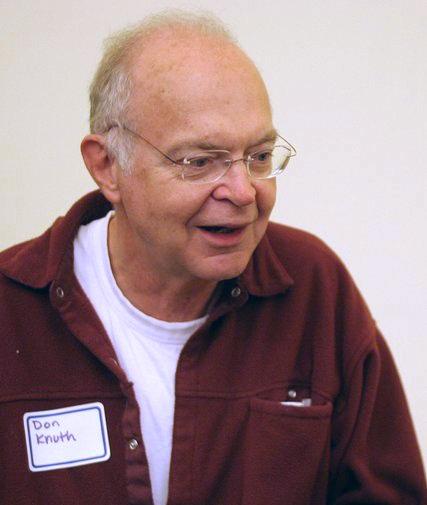
\includegraphics[scale=.5]{imagens/knuth}
    \caption{Donald Knuth em 2005}
  \end{figure}
\end{frame}

\begin{frame}[plain]
  \hspace*{-11.5mm}
  \begin{centering}
    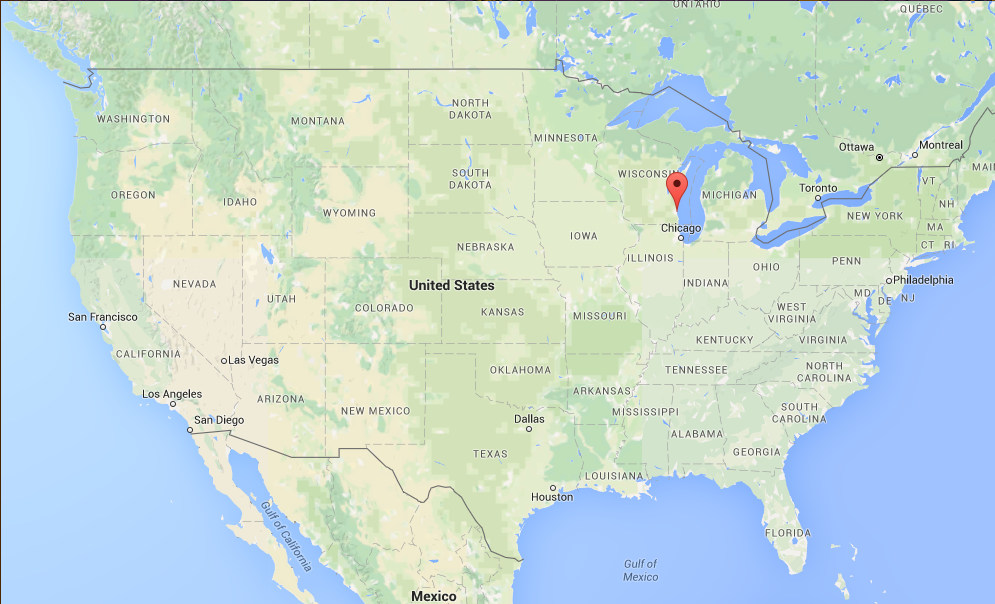
\includegraphics[width=\pagewidth]{imagens/milwaukee}
  \end{centering}
\end{frame}

\begin{frame}
  \frametitle{História do LaTeX}
  \LARGE
  \only<1>{O pai de Knuth\\ tinha uma editora}
  \only<2>{1977: segunda edição do segundo volume de \emph{The Art of Computer
  Programming}}
  \only<3>{\textsc{ascii} não foi projetado\\ com livros em mente}
  \only<4>{\TeX: tau epsilon chi}
\end{frame}

\begin{frame}
  \large
  \begin{quote}
    The purpose of this pronunciation exercise is to remind you that \TeX\ is
    primarily concerned with high-quality technical manuscripts: Its emphasis
    is on art and technology, as in the underlying Greek word. If you merely
    want to produce a passably good document—something acceptable and basically
    readable but not really beautiful—a simpler system will usually suffice.
    With \TeX\ the goal is to produce the finest quality; this requires more
    attention to detail, but you will not find it much harder to go the extra
    distance, and you’ll be able to take special pride in the finished
    product.\hfill (Donald Knuth, \emph{\TeX book})
  \end{quote}
\end{frame}

\begin{frame}
  \frametitle{História do LaTeX}
  \LARGE
  \LaTeX: 1985
\end{frame}

\begin{frame}[plain]
  \begin{figure}[h]
    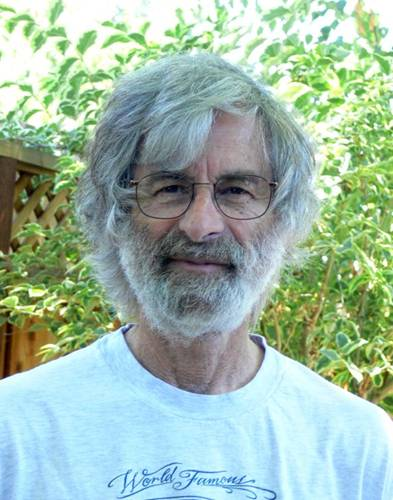
\includegraphics[scale=.5]{imagens/lamport}
    \caption{Leslie Lamport}
  \end{figure}
\end{frame}

% LaTeX: uma linguagem de marcação %%%%%%%%%%%%%%
\section[\LaTeX: uma linguagem de marcação]{Linguagem de marcação}

% O LaTeX é uma linguagem de marcação de texto, ou markup
\begin{frame}
  \frametitle{\LaTeX: uma linguagem de marcação}
  \LARGE
  \only<1>{\LaTeX{} é uma linguagem de \emph{markup}}
  \only<2>{Você \emph{declara} o documento}
  \only<3>{O programa segue as instruções}
  \only<4>{Assim como em \textsc{html},\\ o arquivo fonte é renderizado}
  \only<5>{Comandos são semânticos}
\end{frame}

% Se os comandos são semânticos, devem ser fáceis de interpretar. O que os
% comandos abaixo significam?
\begin{frame}[fragile]
  \frametitle{\LaTeX: uma linguagem de marcação}
  \begin{minted}[autogobble,fontsize=\LARGE,breaklines]{latex}
    \tableofcontents

    \section{Introdução}
  \end{minted}
\end{frame}

% Arquivos .tex não contém formatação; são texto plano.
\begin{frame}
  \frametitle{\LaTeX: uma linguagem de marcação}
  \LARGE
  \code{.tex} são arquivos de texto plano
\end{frame}

\begin{frame}[standout]
  \Huge
  Obrigado!
\end{frame}

\begin{frame}
  \begin{center}
    \vspace{2em}
    
\includegraphics[width=3cm]{imagens/cc}\\
    2016 Alguns direitos reservados para Rafael Beraldo
    \vspace{1em}
    \url{http://creativecommons.org/licenses/by-sa/4.0/}
    \vfill
    \huge{Powered by \LaTeX{}}
  \end{center}
\end{frame}

\end{document}
